\documentclass[aspectratio=169,11pt]{beamer}
\usepackage{beamerucad}
\usepackage{mathtools}
\usepackage{listings}
\definecolor{ckw}{HTML}{2563AB}\definecolor{cst}{HTML}{2E8B57}\definecolor{ccm}{HTML}{8A8F98}
\lstdefinestyle{py}{language=Python,basicstyle=\ttfamily\footnotesize,
 keywordstyle=\color{ckw}\bfseries,stringstyle=\color{cst},commentstyle=\color{ccm}\itshape,
 showstringspaces=false,columns=fullflexible,keepspaces=true,
 backgroundcolor=\color{ucadband!8},frame=leftline,framerule=2.5pt,rulecolor=\color{ucadband},
 xleftmargin=8pt,aboveskip=3pt,belowskip=1pt,basewidth=0.5em}
\lstset{style=py}
\newcommand{\vx}{\mathbf{x}}
\newcommand{\va}{\mathbf{a}}
\newcommand{\vz}{\mathbf{z}}
\newcommand{\vb}{\mathbf{b}}
\newcommand{\vw}{\mathbf{w}}
\newcommand{\vd}{\boldsymbol{\delta}}
\title{Introduction au ML — Séance 10}
\subtitle{Les réseaux de neurones : du neurone à la rétropropagation}
\author{Dr. El Hadji Bassirou TOURÉ}
\institute{Département de Mathématiques et Informatique\\ Faculté des Sciences et Techniques\\ Université Cheikh Anta Diop de Dakar}
\date{}
\setucadfoot{Introduction au ML — Séance 10}
\graphicspath{{figs/}}
\begin{document}

\begin{frame}[plain,noframenumbering]\titlepage\end{frame}

\begin{frame}{Objectifs de la séance}
\begin{ucaddef}[Contenu]
{\small Le \textbf{réseau de neurones} est le modèle le plus emblématique de l'IA moderne. On le construit ici \emph{brique par brique}, sans précipitation : un neurone seul, puis une couche, puis un réseau ; les poids, la matrice de poids, le biais. À chaque étape, on relie l'\emph{image}, le \emph{formalisme} et les \emph{chiffres}.}
\end{ucaddef}
\begin{itemize}\small
  \item Le \textbf{neurone} : un objet déjà connu (la régression logistique de la Séance 6), formalisé et calculé sur des chiffres.
  \item La \textbf{largeur} (plusieurs neurones $=$ une couche) et la \textbf{matrice de poids} $W$, présentée avec de vrais nombres — comme la matrice $X$ de la Séance 3.
  \item La \textbf{profondeur} (empiler des couches) et le décompte des \emph{paramètres}.
  \item L'\textbf{activation} non-linéaire et sa dérivée ; pourquoi elle est indispensable (XOR).
  \item L'\textbf{apprentissage} : la perte, la descente de gradient (Séance 5), et la \textbf{rétropropagation} — dérivée, puis déroulée à la main.
  \item \textbf{En pratique} (\texttt{MLPClassifier}) et le verdict honnête : réseau \emph{contre} méthodes d'ensemble (Séance 8).
\end{itemize}
\end{frame}

% #####################################################################
\section{Le neurone}

\begin{frame}{Le point de départ : un objet déjà connu}
\begin{ucadfront}[De la logistique au neurone]
{\small Le mot « neurone » intimide. Pourtant, la brique de base des réseaux est exactement la \textbf{régression logistique} de la Séance 6 : une somme pondérée des entrées, suivie d'une fonction qui produit la sortie. Rien de nouveau — seulement un vocabulaire et une façon de l'assembler. On part donc de ce socle, et on avance \emph{doucement}.}
\end{ucadfront}
{\small Le plan de la séance suit cette montée graduelle : d'abord \emph{un} neurone (cette section) ; puis plusieurs côte à côte, formant une \emph{couche} (la largeur) ; puis des couches empilées (la profondeur). À chaque étape, on écrit le calcul avec des matrices et on le vérifie sur des chiffres concrets. L'objectif : qu'à la fin, un réseau ne soit plus une boîte noire, mais un empilement de calculs que vous savez refaire à la main.}
\end{frame}

\begin{frame}{L'idée : un neurone, deux gestes}
\begin{ucaddef}[L'idée en une phrase]
{\small Un \textbf{neurone} prend des entrées, en calcule une \emph{somme pondérée} (chaque entrée multipliée par un poids, plus un biais), puis applique une \emph{fonction d'activation} qui produit la sortie.}
\end{ucaddef}
\ucadformula{z = w_1 x_1 + w_2 x_2 + \dots + w_d x_d + b = \vw^\top\vx + b \qquad a = f(z)}
{\small Deux gestes seulement. \textbf{(1)} La somme pondérée $z$ : les poids $w_j$ disent l'importance de chaque entrée, le biais $b$ décale le seuil. \textbf{(2)} L'activation $f$ : elle transforme $z$ en sortie $a$. Quand $f$ est la sigmoïde $\sigma$, ce neurone \emph{est} une régression logistique. Tout le reste de la séance consiste à répéter et empiler ce motif.}
\end{frame}

\begin{frame}{Le neurone, en image et en détail}
\figslide{0.86}{f10_neurone_detail}{Un neurone à trois entrées. Les valeurs $x_j$ (bleu) sont pondérées par les poids $w_j$ (vert, sur les flèches) ; on ajoute le biais $b$ (rouge) ; la somme donne $z$ ; l'activation $f$ produit la sortie $a$. Ici $z = 0{,}5$ et $a = \sigma(0{,}5) = 0{,}62$. Tout le calcul d'un neurone tient dans cette image.}
\end{frame}

\begin{frame}{Le neurone à la main}
\begin{ucadex}[Somme pondérée puis activation, sur des chiffres]
{\small Entrées $\vx = (2;\ 3;\ 1)$, poids $\vw = (0{,}5;\ -1;\ 2)$, biais $b = 0{,}5$.
\[ z = \vw^\top\vx + b = (0{,}5)(2) + (-1)(3) + (2)(1) + 0{,}5 = 1 - 3 + 2 + 0{,}5 = \mathbf{0{,}5}. \]
Puis l'activation. Avec la \textbf{sigmoïde} : $a = \sigma(0{,}5) = \dfrac{1}{1 + e^{-0{,}5}} = \mathbf{0{,}62}$. Avec \textbf{ReLU} : $a = \max(0,\ 0{,}5) = \mathbf{0{,}5}$.}
\end{ucadex}
{\small Lecture : le poids $w_2 = -1$ \emph{pénalise} l'entrée $x_2$ ; le poids $w_3 = 2$ l'amplifie. Le neurone résume les trois entrées en un seul nombre, puis le « presse » entre $0$ et $1$ (sigmoïde) — c'est, au chiffre près, le calcul d'une régression logistique de la Séance 6.}
\end{frame}

\begin{frame}{Le neurone est la régression logistique}
\figslide{0.58}{f10_sigmoide}{La sigmoïde transforme la somme pondérée $z$ en une valeur entre $0$ et $1$, interprétée comme une probabilité. Le point rouge marque notre exemple : $z = 0{,}5 \to a = 0{,}62$. Cette courbe est celle de la Séance 6 — un neurone à activation sigmoïde \emph{est} une régression logistique.}
\end{frame}

\begin{frame}{Exercice — calculer la sortie d'un neurone}
\begin{ucadrec}[Énoncé]
{\small Un neurone à deux entrées, poids $\vw = (1{,}5;\ -2)$, biais $b = 1$. (a) Calculer $z$ pour $\vx = (2;\ 1)$. (b) Donner la sortie avec ReLU. (c) Même question pour $\vx = (0;\ 2)$.}
\end{ucadrec}
\pause
\begin{ucadex}[Correction]
{\small \textbf{(a)} $z = (1{,}5)(2) + (-2)(1) + 1 = 3 - 2 + 1 = \mathbf{2}$. \textbf{(b)} ReLU : $\max(0, 2) = \mathbf{2}$. \textbf{(c)} $z = (1{,}5)(0) + (-2)(2) + 1 = -3$ ; ReLU : $\max(0, -3) = \mathbf{0}$ — le neurone est « éteint » pour cette entrée. C'est tout le rôle de ReLU : laisser passer le positif, bloquer le négatif.}
\end{ucadex}
\end{frame}

% #####################################################################
\section{La largeur : une couche de neurones}

\begin{frame}{Un neurone ne voit qu'une chose}
\begin{ucadfront}[Pourquoi plusieurs neurones]
{\small Un seul neurone produit un seul nombre : il ne capte qu'\emph{un} aspect des données. Pour en saisir plusieurs en parallèle, on place \emph{plusieurs} neurones côte à côte, chacun avec ses propres poids — c'est la \textbf{largeur} d'une couche. Ils reçoivent tous les mêmes entrées, mais en tirent des réponses différentes.}
\end{ucadfront}
{\small Imaginons trois neurones sur les mêmes données patient : l'un pourrait réagir surtout à la fièvre, un autre à la glycémie, un troisième à l'âge — selon leurs poids. Ensemble, ils forment une \textbf{couche} qui décrit l'entrée sous trois angles. La question pratique : comment écrire le calcul de \emph{tous} ces neurones d'un coup, proprement ? La réponse tient en un mot : une \emph{matrice}.}
\end{frame}

\begin{frame}{Une couche, en image}
\figslide{0.80}{f10_couche_largeur}{Quatre entrées alimentent trois neurones (la \emph{largeur} de la couche). Chaque neurone a ses propres poids vers les quatre entrées — d'où $4 \times 3 = 12$ poids, plus $3$ biais. Chaque neurone produit sa sortie $a_j$. La couche transforme $4$ nombres en $3$ nombres.}
\end{frame}

\begin{frame}{L'idée : ranger les poids dans une matrice}
\begin{ucaddef}[L'idée en une phrase]
{\small Les poids de tous les neurones d'une couche se rangent dans une \textbf{matrice de poids} $W$ : \emph{une ligne par neurone}, \emph{une colonne par entrée}. Le calcul de la couche entière s'écrit alors en une seule opération : $\vz = W\vx + \vb$.}
\end{ucaddef}
{\small C'est exactement l'esprit de la \textbf{matrice $X$} de la Séance 3, où chaque ligne était un patient. Ici, chaque ligne de $W$ est un neurone, et le produit matrice-vecteur $W\vx$ calcule \emph{simultanément} les sommes pondérées de tous les neurones. Le vecteur de biais $\vb$ ajoute un biais par neurone. Cette écriture compacte n'est pas qu'une élégance : c'est ce qui rend les réseaux calculables vite, et parallélisables sur une carte graphique.}
\end{frame}

\begin{frame}{La couche, formellement}
\begin{ucaddef}[Définition]
{\small Pour une couche de $m$ neurones recevant $d$ entrées : la matrice $W$ est de taille $m \times d$, le biais $\vb$ de taille $m$. La couche calcule un vecteur $\vz$ de $m$ sommes pondérées, puis applique l'activation composante par composante.}
\end{ucaddef}
\ucadformula{\vz = W\vx + \vb \qquad \va = f(\vz) \qquad W \in \mathbb{R}^{m\times d},\ \vx \in \mathbb{R}^{d},\ \vb \in \mathbb{R}^{m}}
{\small Les dimensions s'enchaînent : $W$ ($m \times d$) fois $\vx$ ($d$) donne $\vz$ ($m$). Chaque \emph{ligne} $i$ de $W$ contient les poids du neurone $i$ ; le produit de cette ligne par $\vx$ donne la somme pondérée $z_i$ de ce neurone. Faire le produit matriciel, c'est faire les $m$ sommes pondérées d'un seul geste. Voyons-le sur de vrais chiffres.}
\end{frame}

\begin{frame}{Du réseau à la matrice : la règle d'indexation}
\begin{ucaddef}[Lire la matrice sur le réseau]
{\small Chaque arête du réseau porte un poids. On les range dans $W$ par une règle simple : le poids de l'\textbf{entrée $j$} vers le \textbf{neurone $i$} se place en \emph{ligne $i$, colonne $j$}. Une ligne $=$ un neurone ; une colonne $=$ une entrée.}
\end{ucaddef}
\begin{columns}[c]
\begin{column}{0.52\textwidth}
\centering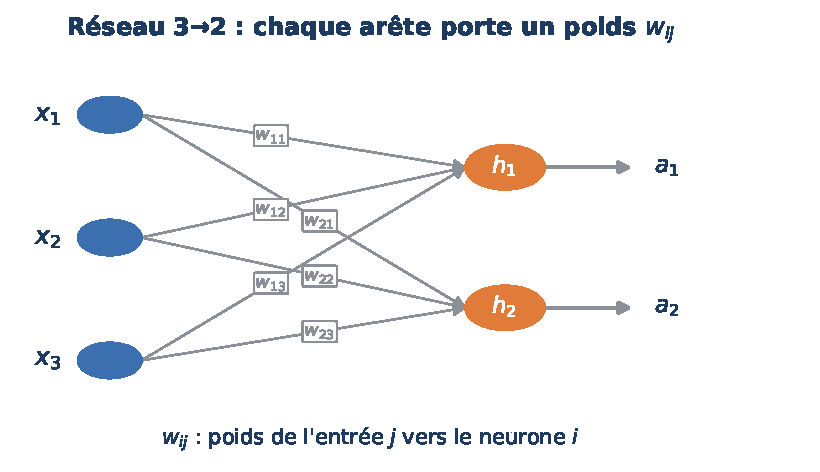
\includegraphics[width=\linewidth,height=0.46\textheight,keepaspectratio]{f10_reseau_sym}
\end{column}
\begin{column}{0.46\textwidth}
{\footnotesize \[ W = \begin{pmatrix} w_{11} & w_{12} & w_{13}\\ w_{21} & w_{22} & w_{23} \end{pmatrix} \]}
{\scriptsize Ligne $1$ : les poids du neurone $h_1$ (vers les $3$ entrées). Ligne $2$ : ceux de $h_2$. Le poids $w_{ij}$ relie l'entrée $j$ au neurone $i$.}
\end{column}
\end{columns}
\end{frame}

\begin{frame}{Du réseau à la matrice : les chiffres}
\begin{ucadex}[On lit $W$ directement sur les arêtes]
{\small Le même réseau $3 \to 2$, avec ses vrais poids. Entrée $\vx = (2;\ 1;\ 0)$, biais $\vb = (0{,}5;\ -1)$.}
\end{ucadex}
\begin{columns}[c]
\begin{column}{0.50\textwidth}
\centering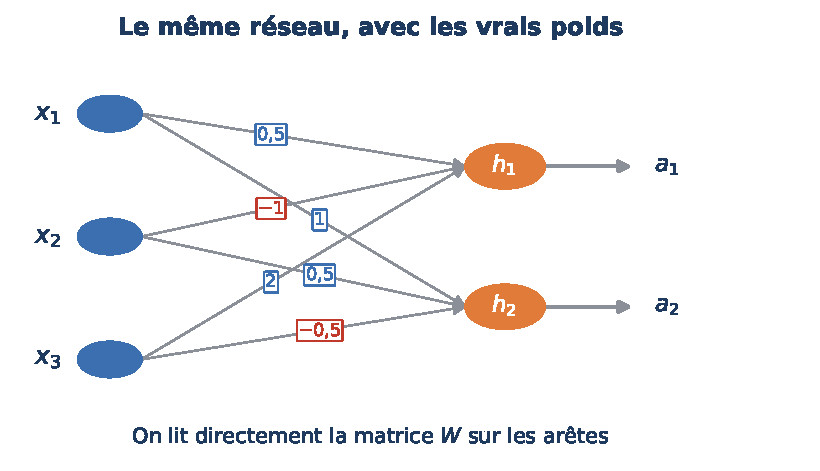
\includegraphics[width=\linewidth,height=0.44\textheight,keepaspectratio]{f10_reseau_num}
\end{column}
\begin{column}{0.48\textwidth}
{\footnotesize \[ W = \begin{pmatrix} 0{,}5 & -1 & 2\\ 1 & 0{,}5 & -0{,}5 \end{pmatrix},\quad \vb = \begin{pmatrix} 0{,}5\\ -1 \end{pmatrix} \]}
{\scriptsize $\vz = W\vx + \vb$ :
\begin{itemize}\setlength\itemsep{1pt}
  \item $z_1 = (0{,}5)(2) + (-1)(1) + (2)(0) + 0{,}5 = \mathbf{0{,}5}$
  \item $z_2 = (1)(2) + (0{,}5)(1) + (-0{,}5)(0) - 1 = \mathbf{1{,}5}$
\end{itemize}
puis $\va = \sigma(\vz) = (0{,}62;\ 0{,}82)$.}
\end{column}
\end{columns}
\end{frame}

\begin{frame}{La matrice de poids, avec de vrais chiffres}
\begin{ucadex}[Comme la matrice $X$ de la Séance 3]
{\small Une couche de $3$ neurones sur $4$ entrées. Entrée $\vx = (1;\ 2;\ 0;\ 3)$, biais $\vb = (0{,}5;\ -1;\ 1)$ :
{\footnotesize \[ W = \begin{pmatrix} 0{,}5 & -1 & 2 & 0\\ 1 & 0{,}5 & -0{,}5 & 1\\ -1 & 2 & 0 & 0{,}5 \end{pmatrix}\!\!\begin{matrix}\ \leftarrow\text{neurone 1}\\ \ \leftarrow\text{neurone 2}\\ \ \leftarrow\text{neurone 3}\end{matrix} \qquad \vx = \begin{pmatrix} 1\\ 2\\ 0\\ 3 \end{pmatrix},\ \vb = \begin{pmatrix} 0{,}5\\ -1\\ 1 \end{pmatrix} \]}
Chaque ligne est un neurone, chaque colonne une entrée. Le produit $W\vx + \vb$ donne les trois sommes pondérées en une fois.}
\end{ucadex}
\end{frame}

\begin{frame}{La matrice de poids, en image}
\figslide{0.66}{f10_matrice_W}{La matrice $W$ ($3 \times 4$) : en bleu les poids positifs, en rouge les négatifs, en gris les nuls. À droite, le vecteur d'entrée $\vx$ et le vecteur de biais $\vb$. Le produit $W\vx + \vb$ calcule les trois sorties $\vz = (-1;\ 4;\ 5{,}5)$ d'un seul coup. C'est le pendant, pour les poids, de la matrice $X$ de la Séance 3.}
\end{frame}

\begin{frame}{Le calcul de la couche, terme à terme}
\begin{ucadex}[$\vz = W\vx + \vb$, ligne par ligne]
{\small Avec $\vx = (1;\ 2;\ 0;\ 3)$ et $\vb = (0{,}5;\ -1;\ 1)$ :
\begin{itemize}
  \item \textbf{neurone 1} : $(0{,}5)(1) + (-1)(2) + (2)(0) + (0)(3) + 0{,}5 = -1{,}5 + 0{,}5 = \mathbf{-1}$.
  \item \textbf{neurone 2} : $(1)(1) + (0{,}5)(2) + (-0{,}5)(0) + (1)(3) - 1 = 5 - 1 = \mathbf{4}$.
  \item \textbf{neurone 3} : $(-1)(1) + (2)(2) + (0)(0) + (0{,}5)(3) + 1 = 4{,}5 + 1 = \mathbf{5{,}5}$.
\end{itemize}
Donc $\vz = (-1;\ 4;\ 5{,}5)$, puis $\va = \sigma(\vz) = (0{,}27;\ 0{,}98;\ 1{,}00)$. La couche a transformé $4$ entrées en $3$ activations — chaque neurone répondant différemment selon ses poids.}
\end{ucadex}
\end{frame}

\begin{frame}{Exercice — le calcul d'un neurone dans une couche}
\begin{ucadrec}[Énoncé]
{\small Reprenons la matrice $W$ ci-dessus et $\vx = (1;\ 2;\ 0;\ 3)$, $\vb = (0{,}5;\ -1;\ 1)$. On ajoute un quatrième neurone, de poids $(2;\ 0;\ 1;\ -1)$ et de biais $0$. Calculer sa somme pondérée $z_4$, puis sa sortie sigmoïde.}
\end{ucadrec}
\pause
\begin{ucadex}[Correction]
{\small $z_4 = (2)(1) + (0)(2) + (1)(0) + (-1)(3) + 0 = 2 - 3 = \mathbf{-1}$. Sortie : $\sigma(-1) = \mathbf{0{,}27}$. Pour l'ajouter à la couche, il suffit d'ajouter une \emph{ligne} $(2, 0, 1, -1)$ à $W$ (qui devient $4 \times 4$) et une composante $0$ à $\vb$. Élargir une couche $=$ ajouter des lignes à $W$.}
\end{ucadex}
\end{frame}

% #####################################################################
\section{La profondeur : empiler les couches}

\begin{frame}{De la largeur à la profondeur}
\begin{ucadfront}[Empiler pour enrichir]
{\small Une couche transforme des entrées en activations. Et si l'on \emph{réinjectait} ces activations dans une \emph{autre} couche ? C'est la \textbf{profondeur} : empiler les couches, la sortie de l'une devenant l'entrée de la suivante. Chaque couche construit des représentations un peu plus élaborées que la précédente.}
\end{ucadfront}
{\small On distingue ainsi la \textbf{largeur} (le nombre de neurones \emph{dans} une couche) et la \textbf{profondeur} (le nombre de couches \emph{empilées}). Un réseau « profond » a beaucoup de couches — d'où le terme \emph{apprentissage profond}. La structure typique : une couche d'entrée (les variables), une ou plusieurs couches \emph{cachées} (au milieu), une couche de sortie (la prédiction). Calculer la prédiction, c'est traverser ces couches de gauche à droite : la \emph{propagation avant}.}
\end{frame}

\begin{frame}{Un réseau, en image}
\figslide{0.80}{f10_profondeur}{Un réseau $4\!-\!3\!-\!1$ : quatre entrées, une couche cachée de trois neurones, une sortie. Chaque couche a sa matrice de poids : $W^{[1]}$ ($3 \times 4$) puis $W^{[2]}$ ($1 \times 3$). La \emph{profondeur} est le nombre de couches (ici $2$) ; la \emph{largeur} de la couche cachée est $3$.}
\end{frame}

\begin{frame}{La propagation avant, formellement}
\begin{ucaddef}[Définition]
{\small On note $\va^{[0]} = \vx$ les entrées. Chaque couche $\ell$ a sa matrice $W^{[\ell]}$ et son biais $\vb^{[\ell]}$, et calcule à partir de la couche précédente :}
\end{ucaddef}
\ucadformula{\vz^{[\ell]} = W^{[\ell]}\va^{[\ell-1]} + \vb^{[\ell]} \qquad \va^{[\ell]} = f\big(\vz^{[\ell]}\big)}
{\small On enchaîne : $\vx \to (\vz^{[1]}, \va^{[1]}) \to (\vz^{[2]}, \va^{[2]}) \to \dots \to \va^{[L]} = \hat y$. Chaque couche fait ses deux gestes — combinaison linéaire $W\va + \vb$, puis activation $f$. La sortie de la dernière couche est la prédiction. Un réseau, en propagation avant, n'est donc qu'une \textbf{composition} de couches : linéaire, activation, linéaire, activation, et ainsi de suite.}
\end{frame}

\begin{frame}{Un réseau profond, ce sont des matrices (en chiffres)}
\begin{ucadex}[Le même principe que la couche, empilé]
{\small Un réseau $2\!-\!2\!-\!1$ avec ses vrais poids. Comme pour une couche, chaque jeu de poids est une \emph{matrice} : $W^{[1]}$ pour la couche cachée, $W^{[2]}$ pour la sortie.}
\end{ucadex}
\begin{columns}[c]
\begin{column}{0.54\textwidth}
\centering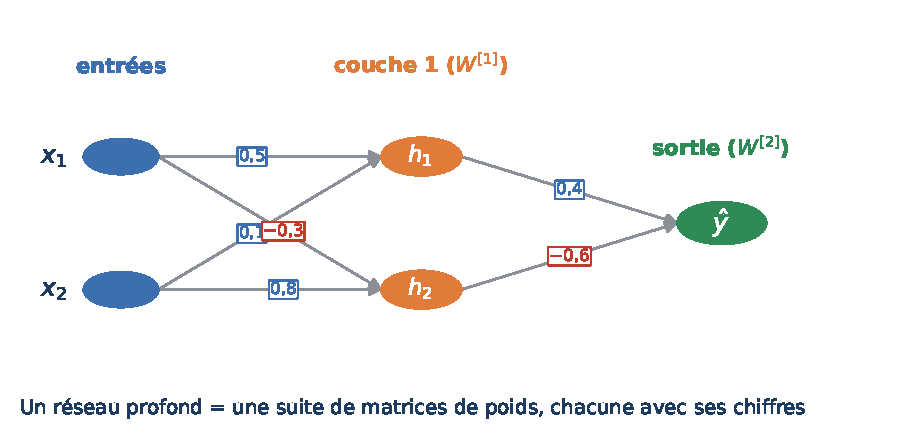
\includegraphics[width=\linewidth,height=0.44\textheight,keepaspectratio]{f10_reseau_profond_num}
\end{column}
\begin{column}{0.44\textwidth}
{\footnotesize \[ W^{[1]} = \begin{pmatrix} 0{,}5 & 0{,}1\\ -0{,}3 & 0{,}8 \end{pmatrix}\!,\ \ W^{[2]} = \begin{pmatrix} 0{,}4 & -0{,}6 \end{pmatrix} \]}
{\scriptsize $W^{[1]}$ est $2\times 2$ (2 neurones, 2 entrées) ; $W^{[2]}$ est $1\times 2$ (1 sortie, 2 neurones cachés). Prédire $=$ enchaîner $\vz^{[1]} = W^{[1]}\vx + \vb^{[1]}$ puis $\hat y = \sigma(W^{[2]}\va^{[1]} + b^{[2]})$. C'est ce réseau que l'on entraînera par rétropropagation.}
\end{column}
\end{columns}
\end{frame}

\begin{frame}{Compter les paramètres d'un réseau}
\begin{ucaddef}[L'idée en une phrase]
{\small Les \textbf{paramètres} d'un réseau sont tous ses poids et tous ses biais — les nombres que l'apprentissage devra ajuster. On les compte couche par couche : pour une couche de $m$ neurones sur $d$ entrées, $m \times d$ poids et $m$ biais.}
\end{ucaddef}
{\small Ce décompte importe : c'est le nombre de « boutons » que la descente de gradient devra régler. Plus il est grand, plus le réseau est expressif, mais plus il est lent à entraîner et enclin au sur-apprentissage (Séances 3 et 7). Sur notre petit réseau $4\!-\!3\!-\!1$, comptons précisément.}
\end{frame}

\begin{frame}{Le décompte, sur le réseau $4\!-\!3\!-\!1$}
\figslide{0.62}{f10_params}{Couche cachée : $W^{[1]}$ a $3 \times 4 = 12$ poids, plus $3$ biais $= 15$. Couche de sortie : $W^{[2]}$ a $1 \times 3 = 3$ poids, plus $1$ biais $= 4$. Total : $\mathbf{19}$ paramètres. Pour un si petit réseau, déjà $19$ nombres à apprendre — d'où l'explosion dès qu'on agrandit, et le besoin d'une méthode automatique d'ajustement.}
\end{frame}

\begin{frame}{Exercice — dimensions et paramètres}
\begin{ucadrec}[Énoncé]
{\small Un réseau a $5$ entrées, une couche cachée de $10$ neurones, une seconde couche cachée de $4$ neurones, et $1$ sortie. (a) Quelle est la taille de chaque matrice de poids ? (b) Combien de paramètres au total (poids $+$ biais) ?}
\end{ucadrec}
\pause
\begin{ucadex}[Correction]
{\small \textbf{(a)} $W^{[1]}$ : $10 \times 5$ ; $W^{[2]}$ : $4 \times 10$ ; $W^{[3]}$ : $1 \times 4$. \textbf{(b)} Poids : $50 + 40 + 4 = 94$. Biais : $10 + 4 + 1 = 15$. Total : $\mathbf{109}$ paramètres. On voit l'explosion : un réseau modeste dépasse déjà la centaine de paramètres — impossible de les régler à la main, d'où la descente de gradient et la rétropropagation.}
\end{ucadex}
\end{frame}

% #####################################################################
\section{La non-linéarité}

\begin{frame}{Pourquoi un seul neurone ne suffit pas}
\begin{ucadfront}[La limite de la frontière droite]
{\small Un seul neurone, comme la logistique, ne trace qu'une \textbf{frontière droite} (Séance 6). Dès que la séparation doit \emph{courber}, il échoue. L'exemple canonique : le \textbf{XOR}, quatre points en damier qu'aucune droite ne sépare. Historiquement, c'est ce test qui a révélé la nécessité des couches cachées \emph{et} de la non-linéarité.}
\end{ucadfront}
{\small Le XOR (« ou exclusif ») vaut $1$ si \emph{exactement une} entrée vaut $1$. Les deux points de classe $1$ sont en diagonale, comme les deux de classe $0$ : aucune droite ne fonctionne. Une régression logistique y atteint $50\,\%$ d'accuracy (le hasard) ; un réseau à une couche cachée atteint $100\,\%$. Mais attention : la couche cachée ne suffit pas seule — encore faut-il une \emph{activation non-linéaire}, comme on va le voir.}
\end{frame}

\begin{frame}{XOR : un neurone échoue, une couche réussit}
\figslide{0.80}{f10_xor}{À gauche, un neurone ne dispose que d'une droite : deux points seront toujours mal classés. À droite, une couche cachée combine plusieurs droites en une frontière \emph{courbe} qui isole chaque classe. C'est l'apport conjoint de la couche cachée et de la non-linéarité.}
\end{frame}

\begin{frame}{L'idée : sans activation, tout s'effondre}
\begin{ucaddef}[L'idée en une phrase]
{\small La \textbf{fonction d'activation} doit être \emph{non-linéaire}. Sans elle, empiler des couches ne sert à rien : la composition de transformations linéaires est \emph{encore} linéaire — le réseau profond se réduit à un unique neurone.}
\end{ucaddef}
{\small C'est le point le plus contre-intuitif de la séance. On pourrait croire qu'empiler deux couches \emph{linéaires} (somme pondérée sans activation) enrichit le modèle. Il n'en est rien. Démontrons-le sur des matrices — c'est court, et cela éclaire \emph{pourquoi} l'activation existe.}
\end{frame}

\begin{frame}{La preuve : deux couches linéaires $=$ une seule}
\begin{ucadex}[Composition linéaire]
{\small Deux couches \emph{sans} activation : $\va^{[1]} = W^{[1]}\vx + \vb^{[1]}$, puis $\hat y = W^{[2]}\va^{[1]} + \vb^{[2]}$. En substituant :
\[ \hat y = W^{[2]}\big(W^{[1]}\vx + \vb^{[1]}\big) + \vb^{[2]} = \underbrace{\big(W^{[2]}W^{[1]}\big)}_{W_{\text{eq}}}\vx + \underbrace{\big(W^{[2]}\vb^{[1]} + \vb^{[2]}\big)}_{\vb_{\text{eq}}}. \]
C'est une \emph{unique} couche linéaire. Vérifié : avec $W^{[1]} = \begin{psmallmatrix} 2 & 1\\ 0 & 3 \end{psmallmatrix}$, $W^{[2]} = \begin{psmallmatrix} 1 & -2 \end{psmallmatrix}$, $\vx = (1; 2)$, les deux couches donnent $-4{,}5$, exactement comme la couche équivalente ($W_{\text{eq}} = \begin{psmallmatrix} 2 & -5 \end{psmallmatrix}$). \textbf{Empiler du linéaire n'apporte rien} : il faut une activation non-linéaire entre les couches.}
\end{ucadex}
\end{frame}

\begin{frame}{Les activations et leurs dérivées}
\figslide{0.86}{f10_activations}{À gauche, trois activations : \textbf{sigmoïde} ($0$ à $1$), \textbf{tanh} ($-1$ à $1$), \textbf{ReLU} ($\max(0,z)$). À droite, leurs \emph{dérivées}, qui interviendront dans la rétropropagation : $\sigma' = a(1-a)$ (plafonne à $0{,}25$), $\tanh' = 1 - a^2$, $\text{ReLU}' = 1$ si $z > 0$ sinon $0$. La faible dérivée de la sigmoïde explique qu'elle « écrase » les gradients en profondeur.}
\end{frame}

\begin{frame}{Pourquoi ReLU domine}
\begin{ucadret}[La plus simple est la meilleure]
\begin{itemize}\small
  \item \textbf{Coût} : un simple test « $z > 0$ ? », bien plus rapide qu'une exponentielle — décisif avec des millions de neurones.
  \item \textbf{Gradients} : sa dérivée vaut $1$ pour $z > 0$, ce qui laisse l'erreur se propager sur de nombreuses couches. La sigmoïde, dont la dérivée plafonne à $0{,}25$, étouffe le gradient en profondeur.
  \item \textbf{Parcimonie} : elle éteint les neurones négatifs (sortie $0$), rendant le réseau plus efficace.
\end{itemize}
\end{ucadret}
{\small En pratique : \textbf{ReLU} dans les couches cachées, \textbf{sigmoïde} en sortie pour une classification binaire. C'est le réglage par défaut, et il fonctionne presque toujours.}
\end{frame}

\begin{frame}{Piège — oublier la non-linéarité}
\begin{ucadpiege}[Un réseau « linéaire » n'apprend rien de plus]
{\small Un réseau à plusieurs couches \emph{sans} activation (ou avec une activation linéaire) donne l'illusion de la puissance, mais se réduit à une régression linéaire ordinaire — incapable de résoudre XOR ou tout motif courbe. La non-linéarité n'est pas un détail : c'est \emph{la} raison d'être des couches.}
\end{ucadpiege}
{\small Corollaire : la profondeur n'a de sens qu'avec des activations non-linéaires. Quand on dit qu'un réseau est « profond », ce qui compte n'est pas seulement le nombre de couches, mais le fait que chacune introduit une non-linéarité qui enrichit ce que le réseau peut représenter.}
\end{frame}

% #####################################################################
\section{L'apprentissage : la perte et le gradient}

\begin{frame}{Apprendre, c'est ajuster les poids}
\begin{ucadfront}[Le problème de l'apprentissage]
{\small Jusqu'ici, les poids étaient \emph{donnés}. Mais d'où viennent-ils ? De l'\textbf{apprentissage} : on part de poids aléatoires, et on les ajuste pour que les prédictions $\hat y$ collent aux vraies étiquettes $y$. Il faut donc deux choses : une mesure de l'erreur (la \emph{perte}), et une méthode pour la réduire (la \emph{descente de gradient}, Séance 5).}
\end{ucadfront}
{\small La logique est exactement celle de la régression linéaire (S5) et logistique (S6) : définir une perte, puis descendre sa pente. La seule difficulté \emph{propre} aux réseaux est calculatoire : comment obtenir la dérivée de la perte par rapport à \emph{chacun} des nombreux poids, y compris ceux des couches cachées ? La réponse — la rétropropagation — viendra à la section suivante. D'abord, la perte.}
\end{frame}

\begin{frame}{La perte : l'entropie croisée}
\begin{ucaddef}[Définition]
{\small Pour une classification binaire, la sortie $\hat y \in [0,1]$ est la probabilité prédite que $y = 1$. La \textbf{perte d'entropie croisée} (déjà vue en Séance 6, issue du maximum de vraisemblance) mesure l'écart entre $\hat y$ et $y$ :}
\end{ucaddef}
\ucadformula{L(y, \hat y) = -\big[\, y \ln \hat y + (1-y)\ln(1-\hat y)\,\big]}
{\small Lecture : si $y = 1$, la perte vaut $-\ln \hat y$ — nulle quand $\hat y \to 1$, énorme quand $\hat y \to 0$ (le modèle est puni d'être confiant et faux). Symétriquement si $y = 0$. Sur notre futur exemple ($y = 1$, $\hat y = 0{,}558$) : $L = -\ln(0{,}558) = 0{,}584$. Cette perte est différentiable — c'est ce qui permet la descente de gradient.}
\end{frame}

\begin{frame}{La descente de gradient, formellement}
\begin{ucaddef}[L'idée en une phrase]
{\small On ajuste chaque poids dans la direction \emph{opposée} à sa dérivée partielle de la perte, d'un petit pas $\eta$ (le taux d'apprentissage), et l'on répète. C'est la méthode de la Séance 5, appliquée à tous les poids du réseau.}
\end{ucaddef}
\ucadformula{w \;\leftarrow\; w - \eta\,\frac{\partial L}{\partial w} \qquad \text{(pour \emph{chaque} poids et biais)}}
{\small Descendre la pente de la perte, exactement comme pour la régression linéaire. Le taux $\eta$ règle la taille du pas : trop grand, on diverge ; trop petit, on traîne. La seule pièce manquante est le calcul de $\partial L / \partial w$ pour les \emph{milliers} de poids du réseau — et c'est précisément ce que résout la rétropropagation, qu'on aborde maintenant.}
\end{frame}

% #####################################################################
\section{La rétropropagation}

\begin{frame}{Le défi : des milliers de dérivées}
\begin{ucadpiege}[Le calcul naïf est impraticable]
{\small Il faut $\partial L / \partial w$ pour \emph{chaque} poids. Les recalculer un à un, en refaisant tout le réseau à chaque fois, coûterait un temps prohibitif : le réseau serait inentraînable. Il faut une méthode qui obtient \emph{tous} les gradients efficacement.}
\end{ucadpiege}
{\small La clé : ces dérivées partagent d'énormes quantités de calcul. La \textbf{rétropropagation} les obtient toutes en une seule passe arrière, en réutilisant les résultats grâce à la \emph{règle de dérivation en chaîne}. C'est cet algorithme — et lui seul — qui a rendu les réseaux profonds entraînables, et donc possible toute l'IA moderne. On va le dériver, puis le dérouler à la main.}
\end{frame}

\begin{frame}{L'idée : renvoyer l'erreur en arrière}
\begin{ucaddef}[L'idée en une phrase]
{\small La \textbf{rétropropagation} calcule le gradient de la perte par rapport à chaque poids en partant de la \emph{sortie} et en remontant couche par couche vers l'\emph{entrée}, réutilisant à chaque étape l'erreur de la couche suivante.}
\end{ucaddef}
{\small L'image : une erreur constatée en sortie est « renvoyée » à travers le réseau ; chaque couche reçoit sa part de responsabilité — notée $\vd^{[\ell]}$, l'\emph{erreur} de la couche $\ell$ — et en déduit comment corriger ses poids. À chaque itération, deux passes alternent : la propagation \textbf{avant} (calculer $\hat y$ et la perte), puis la propagation \textbf{arrière} (calculer tous les gradients). Établissons les quatre équations de cette passe arrière.}
\end{frame}

\begin{frame}{Les deux passes, en image}
\figslide{0.82}{f10_backprop}{En \textbf{vert}, la propagation avant : l'information va de l'entrée vers la sortie pour produire $\hat y$. En \textbf{rouge}, la rétropropagation : l'erreur $\vd$ remonte de la sortie vers l'entrée, chaque couche ajustant ses poids. Les deux passes s'enchaînent à chaque itération de la descente de gradient.}
\end{frame}

\begin{frame}{L'outil : la règle de dérivation en chaîne}
\begin{ucaddef}[Le seul ingrédient mathématique]
{\small Si une quantité $L$ dépend de $z$, qui dépend de $w$, alors la dérivée de $L$ par rapport à $w$ est le \emph{produit} des dérivées le long du chemin :}
\end{ucaddef}
\ucadformula{\frac{\partial L}{\partial w} = \frac{\partial L}{\partial z}\cdot\frac{\partial z}{\partial w}}
{\small Pour savoir comment un poids \emph{profond} influence la perte, on enchaîne les sensibilités le long du chemin qui les relie. La rétropropagation n'est rien d'autre que l'application \emph{organisée} de cette règle, de la sortie vers l'entrée, en stockant les résultats intermédiaires $\vd^{[\ell]}$ pour ne jamais recalculer deux fois la même chose. Établissons d'abord l'erreur de \emph{sortie}, puis celle des couches \emph{cachées}.}
\end{frame}

\begin{frame}{Dérivation 1 — l'erreur de sortie}
\begin{ucadex}[Le résultat propre $\hat y - y$]
{\small On cherche $\delta^{[L]} = \partial L / \partial z^{[L]}$, avec $\hat y = \sigma(z^{[L]})$ et $L$ l'entropie croisée. Par la règle en chaîne :
\[ \delta^{[L]} = \frac{\partial L}{\partial \hat y}\cdot\frac{\partial \hat y}{\partial z^{[L]}}. \]
Or $\dfrac{\partial L}{\partial \hat y} = \dfrac{\hat y - y}{\hat y(1-\hat y)}$ et $\dfrac{\partial \hat y}{\partial z^{[L]}} = \sigma'(z^{[L]}) = \hat y(1-\hat y)$. En multipliant, le facteur $\hat y(1-\hat y)$ \emph{se simplifie} :
\[ \boxed{\;\delta^{[L]} = \hat y - y\;} \]
L'erreur de sortie est juste l'\emph{écart} prédiction $-$ vérité. Toute la complexité s'annule — c'est pourquoi le couple sigmoïde $+$ entropie croisée s'est imposé.}
\end{ucadex}
\end{frame}

\begin{frame}{Dérivation 2 — l'erreur d'une couche cachée}
\begin{ucadex}[Remonter l'erreur, couche par couche]
{\small Pour une couche cachée $\ell$, l'erreur $\vd^{[\ell]} = \partial L / \partial \vz^{[\ell]}$ se déduit de celle de la couche \emph{suivante}. Intuition : $\vz^{[\ell]}$ influence la perte \emph{à travers} la couche $\ell+1$. La règle en chaîne donne, en propageant via les poids puis l'activation :
\[ \boxed{\;\vd^{[\ell]} = \big(W^{[\ell+1]}\big)^\top \vd^{[\ell+1]} \,\odot\, f'\!\big(\vz^{[\ell]}\big)\;} \]
Deux gestes : \textbf{(1)} $\big(W^{[\ell+1]}\big)^\top \vd^{[\ell+1]}$ « renvoie » l'erreur de la couche suivante vers la couche $\ell$ (transposée des poids) ; \textbf{(2)} $\odot\, f'(\vz^{[\ell]})$ la module par la pente locale de l'activation ($\odot$ : produit composante par composante). C'est ici qu'intervient la \emph{dérivée} de l'activation.}
\end{ucadex}
\end{frame}

\begin{frame}{Les quatre équations de la rétropropagation}
\begin{ucadret}[Tout le backprop tient en quatre lignes]
{\small \begin{align*}
\textbf{(1)}\quad & \delta^{[L]} = \hat y - y && \text{erreur de sortie}\\[2pt]
\textbf{(2)}\quad & \vd^{[\ell]} = \big(W^{[\ell+1]}\big)^\top \vd^{[\ell+1]} \odot f'(\vz^{[\ell]}) && \text{erreur rétropropagée}\\[2pt]
\textbf{(3)}\quad & \frac{\partial L}{\partial W^{[\ell]}} = \vd^{[\ell]} \big(\va^{[\ell-1]}\big)^\top && \text{gradient des poids}\\[2pt]
\textbf{(4)}\quad & \frac{\partial L}{\partial \vb^{[\ell]}} = \vd^{[\ell]} && \text{gradient des biais}
\end{align*}}
\end{ucadret}
{\small (1)–(2) : calculer les erreurs, de la sortie vers l'entrée. (3)–(4) : en déduire les gradients de tous les poids et biais. C'est \emph{tout} l'algorithme. Appliquons-le maintenant, en chiffres.}
\end{frame}

% #####################################################################
\section{Un pas de rétropropagation à la main}

\begin{frame}{Le réseau et la propagation avant}
\begin{ucadex}[Un réseau $2\!-\!2\!-\!1$ en chiffres]
{\small Poids : $W^{[1]} = \begin{psmallmatrix} 0{,}5 & 0{,}1\\ -0{,}3 & 0{,}8 \end{psmallmatrix}$, $\vb^{[1]} = (0{,}1;\ -0{,}2)$, $W^{[2]} = (0{,}4;\ -0{,}6)$, $b^{[2]} = 0{,}2$. Entrée $\vx = (1;\ 0)$, cible $y = 1$.
\begin{itemize}
  \item $\vz^{[1]} = W^{[1]}\vx + \vb^{[1]} = (0{,}6;\ -0{,}5)$, \quad $\va^{[1]} = \sigma(\vz^{[1]}) = (0{,}646;\ 0{,}378)$.
  \item $z^{[2]} = W^{[2]}\va^{[1]} + b^{[2]} = 0{,}232$, \quad $\hat y = \sigma(0{,}232) = \mathbf{0{,}558}$.
  \item perte $L = -\ln(0{,}558) = \mathbf{0{,}584}$.
\end{itemize}
La prédiction $0{,}558$ est loin de la cible $1$ : la perte est élevée. La passe arrière va dire comment corriger chaque poids.}
\end{ucadex}
\end{frame}

\begin{frame}{La passe arrière — erreurs et gradients}
\begin{ucadex}[Application des quatre équations]
{\small \textbf{Éq. 1 — erreur de sortie} : $\delta^{[2]} = \hat y - y = 0{,}558 - 1 = \mathbf{-0{,}442}$.

\textbf{Éq. 3–4 — gradients de la sortie} :
\[ \frac{\partial L}{\partial W^{[2]}} = \delta^{[2]}\va^{[1]} = -0{,}442\,(0{,}646;\ 0{,}378) = (-0{,}286;\ -0{,}167), \quad \frac{\partial L}{\partial b^{[2]}} = -0{,}442. \]

\textbf{Éq. 2 — erreur rétropropagée} : $\vd^{[1]} = (W^{[2]})^\top \delta^{[2]} \odot \sigma'(\vz^{[1]}) = (-0{,}040;\ 0{,}062)$.

\textbf{Éq. 3–4 — gradients de la couche cachée} : $\dfrac{\partial L}{\partial W^{[1]}} = \vd^{[1]}\vx^\top = \begin{psmallmatrix} -0{,}040 & 0\\ 0{,}062 & 0 \end{psmallmatrix}$, $\dfrac{\partial L}{\partial \vb^{[1]}} = (-0{,}040;\ 0{,}062)$.}
\end{ucadex}
\end{frame}

\begin{frame}{Vérification : différences finies}
\begin{ucadret}[La dérivation est-elle correcte ?]
{\small Pour être \emph{sûr} de ces gradients, on les recalcule \emph{indépendamment}, sans backprop, par la définition même de la dérivée — la \textbf{différence finie} : faire varier un poids de $\varepsilon$ minuscule, mesurer la variation de perte, diviser.}
\end{ucadret}
\ucadformula{\frac{\partial L}{\partial w} \approx \frac{L(w+\varepsilon) - L(w-\varepsilon)}{2\varepsilon} \qquad (\varepsilon = 10^{-6})}
{\small Résultat (vérifié en code) : pour $\partial L/\partial W^{[2]}_1$, le backprop donne $-0{,}28559$ et la différence finie $-0{,}28559$ — écart de $6 \times 10^{-11}$. Idem pour \emph{tous} les autres gradients (écarts $\sim 10^{-10}$). La dérivation des quatre équations est donc \textbf{exacte}. Ce « test du gradient » est le réflexe pour valider toute implémentation de backprop.}
\end{frame}

\begin{frame}{La mise à jour fait baisser la perte}
\begin{ucadex}[Un pas de descente de gradient, $\eta = 0{,}5$]
{\small On applique $w \leftarrow w - \eta\,\partial L/\partial w$ à tous les poids. Par exemple :
\[ W^{[2]} = (0{,}4;\ -0{,}6) \to (0{,}4;\ -0{,}6) - 0{,}5\,(-0{,}286;\ -0{,}167) = (0{,}543;\ -0{,}517). \]
\[ b^{[2]} = 0{,}2 \to 0{,}2 - 0{,}5(-0{,}442) = 0{,}421. \]
Après mise à jour de \emph{tous} les poids, une nouvelle propagation avant donne une perte de $\mathbf{0{,}441}$ — contre $0{,}584$ avant : une baisse de $0{,}143$ en un seul pas. Le réseau a appris. Répété des milliers de fois sur tous les exemples, ce mécanisme entraîne le réseau.}
\end{ucadex}
\end{frame}

\begin{frame}{La perte décroît, comme en Séance 5}
\figduo{0.42}{f10_descente}{0.52}{f10_loss}{À gauche, notre pas à la main : la perte chute de $0{,}584$ à $0{,}441$. À droite, l'entraînement complet d'un réseau sur DataSANTÉ : la perte décroît de $0{,}57$ à $0{,}34$ au fil des itérations, puis se stabilise. C'est, à plus grande échelle, la descente de gradient de la Séance 5.}
\end{frame}

\begin{frame}{Exercice — une étape de rétropropagation}
\begin{ucadrec}[Énoncé]
{\small Un neurone de sortie (sigmoïde) produit $\hat y = 0{,}8$ pour une cible $y = 0$. L'activation cachée précédente est $\va^{[1]} = (0{,}5;\ 1{,}0)$. (a) Calculer $\delta^{[2]} = \hat y - y$. (b) En déduire $\partial L/\partial W^{[2]} = \delta^{[2]}\va^{[1]}$. (c) Le poids $W^{[2]}_1 = 0{,}3$ : après un pas avec $\eta = 0{,}1$, que devient-il ?}
\end{ucadrec}
\pause
\begin{ucadex}[Correction]
{\small \textbf{(a)} $\delta^{[2]} = 0{,}8 - 0 = \mathbf{0{,}8}$ (le modèle prédit fort alors que $y = 0$ : grosse erreur). \textbf{(b)} $\partial L/\partial W^{[2]} = 0{,}8\,(0{,}5;\ 1{,}0) = (0{,}40;\ 0{,}80)$. \textbf{(c)} $W^{[2]}_1 \leftarrow 0{,}3 - 0{,}1(0{,}40) = \mathbf{0{,}26}$ : le poids \emph{diminue}, ce qui réduira la prédiction la prochaine fois — exactement l'effet voulu.}
\end{ucadex}
\end{frame}

\begin{frame}{Piège — l'apprentissage est délicat}
\begin{ucadpiege}[Plus de paramètres, plus de réglages]
{\small Beaucoup de poids $=$ plus de façons de mal apprendre. La descente de gradient peut diverger si $\eta$ est trop grand, stagner s'il est trop petit, ou rester coincée. Les réseaux sont très sensibles à la \textbf{standardisation} des entrées (Séance 9) et à l'\emph{initialisation} des poids.}
\end{ucadpiege}
{\small Conséquences pratiques : \textbf{toujours standardiser} ; surveiller la courbe de perte pour détecter une divergence ; accepter qu'un réseau demande plus de tâtonnement qu'un modèle d'ensemble. Le « gradient évanescent » (sigmoïde qui écrase les gradients en profondeur) est l'une de ces difficultés — et la raison du succès de ReLU.}
\end{frame}

% #####################################################################
\section{En pratique avec scikit-learn}

\begin{frame}[fragile]{En pratique : MLPClassifier}
\begin{lstlisting}
from sklearn.preprocessing import StandardScaler
from sklearn.neural_network import MLPClassifier

X = StandardScaler().fit_transform(df[colonnes])   # OBLIGATOIRE pour un reseau
reseau = MLPClassifier(
    hidden_layer_sizes=(16, 8),  # deux couches cachees : 16 puis 8 neurones
    activation="relu",            # ReLU dans les couches cachees
    max_iter=1000,                # iterations de descente de gradient
    random_state=0)
reseau.fit(X_train, y_train)
print(reseau.score(X_test, y_test))   # accuracy
print(reseau.loss_curve_[-1])         # perte finale
\end{lstlisting}
{\small \texttt{MLP} signifie \emph{Multi-Layer Perceptron} — le nom historique du réseau classique. \texttt{hidden\_layer\_sizes=(16, 8)} décrit deux couches cachées. scikit-learn applique la rétropropagation et la descente de gradient en interne ; vous savez désormais ce qu'elles font. La standardisation préalable n'est pas optionnelle.}
\end{frame}

\begin{frame}{Les réglages qui comptent}
\begin{ucadret}[Quatre leviers principaux]
\begin{itemize}\small
  \item \texttt{hidden\_layer\_sizes} : nombre de couches et de neurones (profondeur et largeur). Plus grand $=$ plus expressif, mais plus lent et plus enclin au sur-apprentissage.
  \item \texttt{activation} : \texttt{"relu"} par défaut pour les couches cachées (le bon choix presque toujours).
  \item \texttt{alpha} : la régularisation $L_2$ (Séance 7) — augmenter contre le sur-apprentissage.
  \item \texttt{learning\_rate\_init} : le taux d'apprentissage $\eta$ — trop grand, ça diverge ; trop petit, ça traîne.
\end{itemize}
\end{ucadret}
{\small À retenir : commencer simple (une ou deux petites couches), standardiser, surveiller la courbe de perte, n'agrandir que si le sous-apprentissage le justifie.}
\end{frame}

\begin{frame}{La taille de la couche : un plafond vite atteint}
\figslide{0.62}{f10_archi}{Sur DataSANTÉ, agrandir la couche cachée ($2 \to 8 \to 16 \to 32$, puis deux couches) ne change \emph{rien} à l'accuracy : elle plafonne à $0{,}882$. La capacité utile dépend de la \emph{complexité des données}, pas de la taille du modèle — et nos données tabulaires n'en demandent pas tant.}
\end{frame}

% #####################################################################
\section{Le verdict : réseau contre ensembles}

\begin{frame}{La question qui fâche}
\begin{ucadfront}[Faut-il un réseau sur nos données ?]
{\small Les réseaux dominent l'actualité — images, traduction, IA générative. La tentation est de les croire \emph{toujours} supérieurs. Confrontons l'idée à nos données : un réseau bat-il les méthodes d'ensemble (Séance 8) sur le paludisme de DataSANTÉ ?}
\end{ucadfront}
{\small On compare, sur le même découpage train/test et avec les mêmes soins (standardisation pour le réseau), quatre modèles : la régression logistique (un neurone, S6), un réseau \texttt{MLP}, une forêt aléatoire et un gradient boosting (S8). Juge : l'AUC sur le test, comme en Séances 6–7.}
\end{frame}

\begin{frame}{Le comparatif honnête}
\figslide{0.64}{f10_verdict}{Les quatre modèles se tiennent dans un mouchoir : gradient boosting $0{,}700$, régression logistique $0{,}698$, réseau $0{,}693$, forêt $0{,}662$. Le réseau ne fait \emph{pas} mieux que la simple régression logistique — et reste derrière le boosting. Pour une complexité et un temps de réglage bien supérieurs, aucun gain.}
\end{frame}

\begin{frame}{La leçon : le réseau n'est pas magique}
\begin{ucadret}[Sur données tabulaires, les ensembles règnent]
{\small Ce résultat n'est pas un accident : c'est un \textbf{fait empirique général}. Sur les données \emph{tabulaires} (lignes et colonnes, comme un tableur médical), les méthodes d'ensemble — forêts, gradient boosting, XGBoost — sont régulièrement aussi bonnes ou meilleures que les réseaux, pour bien moins d'efforts.}
\end{ucadret}
{\small Même leçon de maturité qu'en Séance 8 (« plus puissant n'est pas meilleur »), poussée plus loin : la \emph{popularité} d'une famille de modèles ne dit rien de sa pertinence pour \emph{votre} problème. Choisir un réseau par effet de mode, sur des données qui n'en ont pas besoin, c'est payer cher une complexité inutile.}
\end{frame}

\begin{frame}{Alors, quand le réseau gagne-t-il ?}
\begin{ucaddef}[Le domaine des réseaux]
{\small Les réseaux brillent là où la structure est \emph{riche et non tabulaire} : \textbf{images} (chaque pixel lié à ses voisins), \textbf{texte} et \textbf{son} (séquences), et les problèmes à \emph{très grand volume} de données.}
\end{ucaddef}
{\small Sur ces données, aucune méthode d'ensemble ne rivalise : c'est le territoire naturel de l'apprentissage profond, et la raison de son succès. Règle pratique : \textbf{tabulaire} de taille modeste $\to$ commencer par les ensembles ; \textbf{images, texte, son, très grand volume} $\to$ les réseaux prennent l'avantage. Et c'est précisément ce domaine — convolutions, séquences, transformeurs — que développera le cours de \emph{Deep Learning} au prochain semestre, en s'appuyant sur la rétropropagation établie aujourd'hui.}
\end{frame}

% #####################################################################
\section{Synthèse}

\begin{frame}{Quel modèle pour quel problème}
\begin{ucadret}[Une carte de tout le cours]
{\small \begin{center}\renewcommand{\arraystretch}{1.25}
\begin{tabular}{l|l}
\textbf{situation} & \textbf{modèle de premier choix}\\\hline
relation simple, interprétable & régression linéaire / logistique (S5–S6)\\
données tabulaires, performance & forêt, gradient boosting (S8)\\
structure inconnue à explorer & clustering, PCA (S9)\\
images, texte, son, gros volume & réseaux de neurones (S10)\\
toujours, en premier & le modèle \emph{simple} comme référence\\
\end{tabular}\end{center}}
\end{ucadret}
\end{frame}

\begin{frame}{Le protocole réseau}
\begin{ucadret}[De bout en bout]
{\small \textbf{1.} Se demander si un réseau est \emph{justifié} (tabulaire $\to$ essayer les ensembles d'abord) $\to$ \textbf{2.} \textbf{standardiser}, sans exception $\to$ \textbf{3.} commencer \emph{petit} (une ou deux petites couches, \texttt{relu}) $\to$ \textbf{4.} entraîner et \textbf{surveiller la courbe de perte} $\to$ \textbf{5.} régler si besoin (\texttt{alpha}, taille, $\eta$) $\to$ \textbf{6.} comparer \emph{honnêtement} à une référence simple : si le réseau ne fait pas mieux, garder le modèle simple.}
\end{ucadret}
\end{frame}

\begin{frame}{À retenir — Séance 10 (1/2)}
\begin{ucadret}[Du neurone au réseau]
\begin{itemize}\small
  \item Un \textbf{neurone} $=$ somme pondérée $z = \vw^\top\vx + b$ suivie d'une activation $f(z)$ : c'est la régression logistique (S6) quand $f = \sigma$.
  \item La \textbf{largeur} (plusieurs neurones) se range dans une \textbf{matrice de poids} $W$ ($m \times d$, une ligne par neurone) : la couche calcule $\vz = W\vx + \vb$.
  \item La \textbf{profondeur} empile les couches ; prédire $=$ \emph{propagation avant} $\vz^{[\ell]} = W^{[\ell]}\va^{[\ell-1]} + \vb^{[\ell]}$.
  \item L'\textbf{activation non-linéaire} est indispensable (sans elle, empiler $=$ une seule couche linéaire) ; \textbf{ReLU} domine dans les couches cachées.
\end{itemize}
\end{ucadret}
\end{frame}

\begin{frame}{À retenir — Séance 10 (2/2)}
\begin{ucadret}[L'apprentissage et le verdict]
\begin{itemize}\small
  \item La \textbf{perte} (entropie croisée) mesure l'écart $\hat y$ vs $y$ ; sigmoïde $+$ BCE donne $\partial L/\partial z^{[L]} = \hat y - y$.
  \item Un réseau apprend par \textbf{descente de gradient} (S5) ; la \textbf{rétropropagation} calcule tous les gradients en une passe arrière (4 équations, règle de la chaîne).
  \item Le \textbf{test du gradient} (différences finies) valide toute implémentation ; toujours \textbf{standardiser}.
  \item \textbf{Verdict} : sur \emph{tabulaire}, les ensembles (S8) égalent ou battent les réseaux ; le réseau gagne sur \emph{images, texte, son, gros volumes}. Popularité $\neq$ pertinence.
\end{itemize}
\end{ucadret}
\end{frame}

\begin{frame}{Pièges fréquents}
\begin{itemize}\small
  \item Croire qu'un réseau est \emph{toujours} supérieur : sur tabulaire, les ensembles font souvent aussi bien ou mieux.
  \item Oublier de \textbf{standardiser} : un réseau y est très sensible, bien plus qu'une forêt.
  \item Construire un réseau \emph{sans} activation non-linéaire : il se réduit à une régression linéaire.
  \item Confondre largeur et profondeur, ou expressivité et apprentissage : un réseau \emph{peut} tout représenter, encore faut-il \emph{trouver} les poids.
  \item Ne pas surveiller la courbe de perte : on rate une divergence ($\eta$ trop grand) ou une stagnation.
  \item Implémenter un backprop sans le \textbf{test du gradient} : une erreur de dérivation passe inaperçue.
\end{itemize}
\end{frame}

\begin{frame}{Prochaine séance}
\begin{ucadfront}[Séance 11 — Le projet de bout en bout]
{\small La dernière séance n'introduit pas de nouveau modèle : elle \emph{rassemble} tout le cours en un \textbf{projet complet}, du type des compétitions de science des données. Formuler le problème, préparer les données (S4), choisir et comparer des modèles (S3, S5–S10), évaluer honnêtement (S6–S7), interpréter et présenter. C'est le moment de devenir autonome — et l'évaluation se fera sur ce projet.}
\end{ucadfront}
\end{frame}

\begin{frame}{Références}
\begin{itemize}\small
  \item Goodfellow, Bengio, Courville — \emph{Deep Learning}, MIT Press, 2016 (chap. 6 : réseaux et rétropropagation).
  \item Nielsen — \emph{Neural Networks and Deep Learning}, 2015 (dérivation du backprop).
  \item Géron — \emph{Hands-On Machine Learning}, 3\textsuperscript{e} éd., O'Reilly, 2022.
  \item Bishop — \emph{Pattern Recognition and Machine Learning}, Springer, 2006 (chap. 5).
  \item Cours : Stanford CS231n (réseaux) ; University of Washington CSE 446.
\end{itemize}
\end{frame}

\end{document}
